\documentclass[12pt]{elsart}
\usepackage{amsmath}
\usepackage{amssymb}
\usepackage{program}
\newcommand{\field}[1]{\mathbb{#1}}

\usepackage{multicol}

\usepackage{algorithm}
\usepackage{algpseudocode}

\usepackage{graphicx}

\newenvironment{Figure}
  {\par\medskip\noindent\minipage{\linewidth}}
  {\endminipage\par\medskip}

\def\ni{\noindent}
\def\pb{\pagebreak}

%%%%%%%%%%%%

%%%%%%%%%%%%%%%%%%%%%%%%%%%%%%%%%%%%%%%%%Space to make more readable!
%\vspace{10 mm}
%%%%%%%%%%%%%%%%%%%%%%%%%%%%%%%%%%%%%%%%%Take out later!

\begin{document}

\pagestyle{empty}

\begin{center}
\Large  CS3343 Analysis of Algorithms Fall 2017 \\
\large {\bf Homework 7}\\
\normalsize Due 12/05/17 before 11:59pm (Central Time)
\end{center}

%{\bf 1.  Kruskal’s Algorithm (2 points)}
%
%Run Kruskal’s algorithm on the graph $G_1$.   Specifically, show the order in which the edges are added to the solution.

{\bf 1.  Dijkstra’s Algorithm (3 points)}

Run Dijkstra’s algorithm on the graph $G_1$ to compute the shortest paths from $a$ to all of the other vertices.

\begin{multicols}{2}
\begin{Figure}
 \centering
 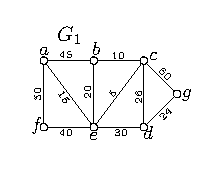
\includegraphics[width=1.1\textwidth]{Graph-01}
\end{Figure}

\begin{tabular}{ |p{0.6cm}|p{0.5cm}|p{0.5cm}|p{0.5cm}|p{0.5cm}|p{0.5cm}|p{0.5cm}|p{0.5cm}| p{0.5cm}| }
  \hline
   $RM$ &  $a$ &  $b$ & $c$ & $d$ & $e$ & $f$ & $g$ \\
  \hline  \hline
  $-$ & 0 & $\infty$ & $\infty$ & $\infty$ & $\infty$ & $\infty$ & $\infty$   \\
 \hline
  $a$ & $-$ & 45 & $\infty$ & $\infty$ & 15 & 50 & $\infty$  \\
  \hline
  $e$ & $-$ & 35 & 20 & 45 & $-$ & 50 & $\infty$ \\
  \hline
  $c$ & $-$ & 30 & $-$ & 45 & $-$ & 50 & 80 \\
  \hline
  $b$ & $-$ & $-$ & $-$ & 45 & $-$ & 50 & 80 \\
  \hline
  $d$ & $-$ & $-$ & $-$ & $-$ & $-$ & 50 & 69 \\
  \hline
  $f$ & $-$ & $-$ & $-$ & $-$ & $-$ & $-$ & 69 \\
  \hline
  $g$ & $-$ & $-$ & $-$ & $-$ & $-$ & $-$ & $-$ \\
  \hline
\end{tabular}

\end{multicols}

{\bf 2.  NP-Hardness Reduction (6 points)}

Let's define a new problem: The satisfiability problem with at most 5 copies of each variable (SAT5C):
\begin{itemize}
  \item Input: a boolean formula $f$ with $m$ clauses over $n$ variables.  No variable appears in more than 5 clauses.
  \item Output: TRUE if there is an assignment to the variables that makes the formula true, FALSE otherwise.
\end{itemize}

\begin{enumerate}
\item (1 point) Is the following boolean formula satisfiable (justify your answer): \\
Yes, setting $x_1 = F$, $x_2 = F$, and $x_3 = F$ \\
{\normalsize $  ( \neg x_3 \vee  x_2) \wedge (x_1 \vee x_3 \vee \neg x_2) \wedge ( \neg x_3 \vee \neg x_2) \wedge (\neg x_1 \vee x_3)  \wedge (x_1 \vee \neg x_3) \wedge ( x_3 \vee \neg x_2)$} \\
{\normalsize $  ( T \vee  F) \wedge (F \vee F \vee T) \wedge (T \vee T) \wedge (T \vee F)  \wedge (F \vee T) \wedge (F \vee T)$} \\
Each clause evaluates to $T$, so the formula evaluates to TRUE.

\item (1 point) Is the above an example of the SAT5C problem?  Why or why not? \\
No, $x_3$ is in 6 clauses, which is greater than the allowable 5 clauses.

\newpage

\item (4 points) Show that $SAT5C$ is NP-hard by giving a polynomial time reduction from $SAT$ to $SAT5C$ (i.e., {\bf $SAT \leq SAT5C$}):

({\bf Hint:} you can ensure two variables have the same truth value by adding 2 additional clauses each of which have two variables in them) 

Given a formula $f$ with $m$ clauses over $n$ variables as input to SAT, a reduction to SAT5C can be constructed trivially if all $n$ variables appear in 5 or less clauses. Otherwise, inputs for SAT5C may be constructed as follows: \\
Let $k$ = the number of appearances of a variable $x_i$ in $f$ \\
$f_{SAT5C} = f_{SAT} \cup m_{SAT5C}$ \\
$m_{SAT5C} = m_{SAT}$ such that each occurrence of $x_i \in n_{SAT} : k > 5$ is replaced by the $k$ new variables in $n_{SAT5C}$ conjoined with, for each new variable $x_j$ for $j = 1,2,...,k - 1$, ($x_j \vee \neg x_{j+1}$), finally conjoined with ($x_{k-1} \vee \neg x_{1}$) \\
$n_{SAT5C} = n_{SAT}$ where for each $x_i \in n_{SAT} : k > 5$ is replaced by $k$ new variables not in $n_{SAT}$ for each of the $k$ appearances of $x_i$


The replacement of a variable with $k >$ 5 appearances with $k$ new variables and the resulting conjunction with the clauses described in $m_{SAT5C}$ results in the removal of the offending variable replaced by $k$ new variables all with $<$ 5 appearances. The additional clauses ensure that each of the new variables have the same truth value (the truth value of the offending variable) because for all clauses in the chain to be true, each of the new variables must have the same truth value.
\end{enumerate}

{\bf 3.  P vs. NP (14 points)}

Once again let's imagine company $X$ has hired you as a software engineer.  In this case, the company has several databases of customer information it manages for its resale business.  

The business tracks items that customers want to sell and ones they want to buy (See example figure 1).  It also tracks ``fair" prices for buying and selling each of the items (See example figure 2).  Naturally the buy price will be higher than the sell price since the company will keep some money a buyer pays as profit.

\begin{figure}[h]
  \caption{Customers and their items }
\begin{tabular}{ |p{1.75cm}|p{2.0cm}|p{1.25cm}|p{2.5cm}|p{2.5cm}|p{2.5cm}|}
  \hline
   Customer Name & Username & Rating &  Date of Birth &  Wants to Sell & Wants to Buy \\
  \hline  \hline
   Kenneth Rosen & KRosen &  50 & 1950/02/03 &  Item \#0980 \par Item \#1063 \par Item \#2048  & Item \#0351 \\
  \hline
   Alonzo Church & LambdaC&  70 & 1903/06/14 &  Item \#1085  & Item \#1702 \par Item \#2048 \\
  \hline
   Stephen Cook & PvsNP &  20 & 1939/12/14 &  none  & Item \#0980 \par Item \#1702 \\
  \hline
   $\vdots$ & $\vdots$& $\vdots$  &  $\vdots$ & $\vdots$  & $\vdots$ \\
  \hline
\end{tabular}
\end{figure}

\begin{figure}[h]
  \caption{Prices of items }
\begin{tabular}{ |p{3cm}|p{6cm}|p{2.15cm}|p{2.15cm}| }
  \hline
   Item \# &  Item Description &  Purchase Price &  Sell Price \\
  \hline  \hline
   Item \#0351 &  Used Discrete Math Text Book &  \$45 & \$20  \\
  \hline
   Item \#0980 &  Used Graphing Calculator &  \$60 & \$27  \\
  \hline
   Item \#1085 &  Used Book of GRE Practice Problems &  \$6 & \$2  \\
  \hline
   $\vdots$ & $\vdots$& $\vdots$  &  $\vdots$ \\
  \hline
\end{tabular}
\end{figure}

Below is a list of features the company wants you to look into adding.  Specifically, identify whether the given problem can be solved in polynomial time.  If it can, give a short description of an algorithm to compute it (feel free to use algorithms and data structures we learned earlier this semester in your justification).  Alternatively, if you believe the problem is NP-hard, give a short justification why (this doesn't need to be a proof but try to point out a similar NP-hard problem).

You can assume there are $n$ people in the Figure 1 database and $m$ items in the Figure 2 database.  You can treat these databases as 2d arrays (there are some additional caveats for working with real databases that we won't worry about here). You can assume each customer's ``Wants to Buy" and ``Wants to Sell" information are stored in linked lists of length at most $m$.

\begin{enumerate}
  \item {\bf Process Transaction I:} For a given item find a customer with it on their sell list.\\
  Assuming constant time to access a customer's info in the first database, by linearly searching through each customers sell list an item may be found in polynomial time. In the worst case using this approach, the item is not on any customer's sell list and thus the algorithm would finish after searching through every customer's sell list in $O(nm)$ time since each of the $n$ customers could potentially have $m$ items on their sell list.
  \item {\bf Process Transaction II:} For a given item find the highest rated customer selling that item.\\
  This requires a simple modification to the first algorithm, where we must search every customer no matter what and, if the item is found in a customer's sell list, update a variable keeping track of the maximum rating found for a customer selling that item. Thus, the running time for this algorithm would also be $O(nm)$ polynomial time.
  \item {\bf Shopping Buddy I:} Check if there are 3 users where each pair of users have at least one item in common which they want to buy. \\\\
{\bf Example:} These 3 people all share at least one item in their buy list\\
 $\{$ Item \#0927, Item \#1085, Item \#2048 $\}$\\
 $\{$ Item \#1085, Item \#1555 $\}$\\
 $\{$ Item \#1555, Item \#1702, Item \#2048, Item \#3730 $\}$\\
  This problem is NP-hard, it is identical to finding a size three clique in a graph. Letting each customer represent a vertex, add an edge between two vertices if they share an item on their buy list. Then we are looking for three vertices where each is adjacent to the other two. This is equivalent to finding a size three clique, so this problem is also NP-hard.

  \item {\bf Shopping Buddy II:} Check if there is a set of $k$ users where each pair of users have at least one item in common which they want to buy. \\
  This is the same problem as Shopping Buddy I except, instead of three users, we are looking for any $k$ of the $n$ users that have at least one item in common on their buy list. Thus, this problem is equivalent to finding a clique of size $k$ and thus also NP-hard.

  \item {\bf Impostor Usernames:} Find all pairs of usernames where they share a subsequence of $k$ characters.\\

 (for a real application $k$ would vary based on the length of the usernames but for the sake of simplicity we are assuming a static value). \\\\
{\bf Example:} Some pairs of names which share at least 5 characters\\
$($ SipserToC, SimpsonToC $)$\\
$($ KRosen2000, JRosen1999 $)$\\
$($ PvsNP, P\_vs\_NP $)$\\
  This is similar to finding the longest common subsequence which is optimized using dynamic programming, except we are trying to find a subsequence of length $k$ between pairs of usernames instead of the longest common subsequence. Using dynamic programming to find the longest common subsequence between two usernames, we can examine the result and see if the LCS is at least $k$. This algorithm runs in $O(st)$ where $s$ and $t$ are the lengths of the two usernames respectively. Since we are search for all pairs of usernames we must do this for every pair of usernames resulting in a runtime of $O(n^2st)$ which is polynomial in runtime. $s$ and $t$ may change between usernames, but it should be insignificant especially if there is a limit to username length.
  
  \newpage

  \item {\bf Equal Trade Problem:} For a given customer check if there is a subset of items that they want to buy which is equal in value to a subset of items they want to sell. \\\\
{\bf Hint: } Check out Knapsack and Subset Sum problems.\\
  This is almost identical to the Subset Sum problem. Given the customer's buy and sell list, create a combined list of both lists while setting the customer's buy values to their respective negatives. Now we are simply looking for a subset of items in this set that will sum to zero, which means that a subset of the buy list is equal in value to a subset of the sell list if there is a subset in the combined list that sums to zero. Since the Subset Sum problem and this one are equivalent and the Subset Sum problem is NP-Complete, then this problem is NP-Hard.

  \item {\bf Gift Exchange:} Check to see if there are $k$ users where every user can give an item from their sell list to another user who has it on their buy list.  All of the $k$ people should give exactly one gift and receive exactly one gift.\\
  Start by building a directed graph where each vertex is a customer, add a directed edge from one customer to another if the furst customer has an item on their sell list that the other has on their buy list. This can be done in polynomial time since there are at most $m$ items of a buy list and for each of those you must check each of the $m$ items of the $n - 1$ other customers for each of the $n$ customers, resulting in a time $O(n^2m^2)$. Then, to solve the problem we simply use DFS to look for a simple cycle of length $k$. If such a cycle exists then there are $k$ users that will all receive exactly one gift and give exactly one gift, which would form a simply cycle in this graphical representation. Since DFS and cycle detection are also polynomial in runtime, this problem may be solved in an overall polynomial runtime.
\end{enumerate}


%\begin{itemize}
%  \item Given a $SAT$ formula $f_2=C_1, \ldots, C_m$ over the variables $x_1,\ldots, x_n$, we need to produce a $SAT5C$ formula $f_1=B_1, \ldots, B_k$ over the variables $y_1,\ldots, y_l$.
%\end{itemize}


\end{document}